Nous pouvons voir ci-dessous le schéma électrique de la bobine reçue. Il s'agit d'un réseau en étoile, avec une bobine centrale et trois branches de longueurs variables. La branche B est connectée à un générateur d'ondes carrées de 1 MHz. La branche A est connectée à une résistance de 50ohms. La branche C est un circuit ouvert.

\begin{figure}[H]
    \centering
    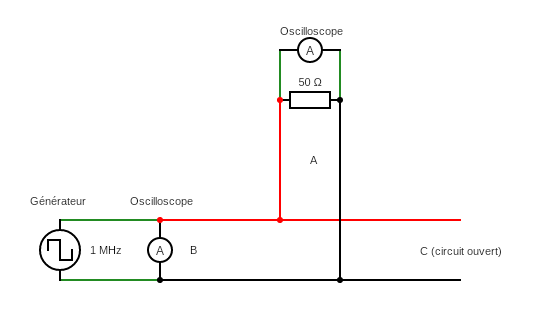
\includegraphics[width=0.7\textwidth]{images/circuit-diagram.png}
    \caption{Schéma électrique du réseau}
    \label{fig:Schema electrique}
\end{figure}
